\documentclass[11pt]{article}
\usepackage[margin=1in]{geometry}
\usepackage{amsmath,amssymb}
\usepackage{graphicx}
\usepackage{booktabs}
\usepackage{siunitx}
\usepackage{hyperref}
\hypersetup{colorlinks=true,linkcolor=blue,urlcolor=blue}
\graphicspath{{../figs/}}

\title{Replication of Stier \textit{et al.} (2017):\\
\emph{Skyrmion--Antiskyrmion Pair Creation by In-Plane Currents}\\
\large arXiv:1701.07256 --- a 2D LLG micromagnetics replication}
\author{Automated replication (TEXTURE-polar-stier2017)}
\date{\today}

\begin{document}
\maketitle

\begin{abstract}
We replicate the central mechanism of Stier \textit{et al.}, PRL/arXiv:1701.07256:
an in-plane spin-polarised current, acting on a chiral-magnet film, drives the
creation of skyrmion--antiskyrmion (Sk--ASk) pairs and, through asymmetric
dissipative decay of one partner, produces a \emph{net change of the total
topological charge} $Q$ (the skyrmion number). We implement a 2D
Landau--Lifshitz--Gilbert (LLG) solver with exchange, interfacial
Dzyaloshinskii--Moriya interaction (DMI), Zeeman coupling, and Zhang--Li
spin-transfer torque (STT), and measure $Q$ with the Berg--L\"uscher lattice
solid-angle method. Two experiments confirm the three sub-claims: (i) a Sk--ASk
pair carries \emph{net-zero} topological charge (charge conservation at
creation); (ii) an in-plane current drives the partners and deflects them
oppositely (skyrmion-Hall effect, the ingredient that separates a pair); and
(iii) the non-DMI-stabilised antiskyrmion \emph{annihilates via Gilbert
damping} while the skyrmion survives, taking the film from $Q=0$ to $Q=-1$
(net $\Delta Q=-1$). \textbf{Verdict: REPLICATED} (core mechanism); the
current-driven \emph{full unbinding} of a bound pair is only partially
demonstrated in our minimal setup.
\end{abstract}

\section{Model and method}
The magnetisation is a unit-vector field $\mathbf n(\mathbf r,t)=\mathbf
M/|\mathbf M|$ on an $N\times N$ square lattice ($N=140$, spacing $=1$). The
energy (Stier Eq.~8, continuum limit) is
\begin{equation}
H = \int \Big[ A(\nabla\mathbf n)^2
   + D\,\big(n_z\,\nabla\!\cdot\!\mathbf n_\perp - (\mathbf n_\perp\!\cdot\!\nabla)n_z\big)
   - B\,n_z \Big]\,d^2r ,
\end{equation}
with exchange stiffness $A$, interfacial (N\'eel) DMI $D$, and perpendicular
Zeeman field $B$. The effective field is $\mathbf B_{\rm eff}=-\partial
H/\partial\mathbf n$, giving on the lattice
\begin{equation}
\mathbf B_{\rm eff}=2A\,\nabla^2\mathbf n
 + 2D\,(\partial_x n_z,\ \partial_y n_z,\ -(\partial_x n_x+\partial_y n_y))
 + B\,\hat{\mathbf z}.
\end{equation}
The dynamics follow the extended LLG equation with in-plane STT,
\begin{equation}
\partial_t\mathbf n = -\mathbf n\times\mathbf B_{\rm eff}
 + \alpha\,\mathbf n\times\partial_t\mathbf n
 + (\mathbf v_s\!\cdot\!\nabla)\mathbf n
 - \beta\,\mathbf n\times(\mathbf v_s\!\cdot\!\nabla)\mathbf n ,
\label{eq:llg}
\end{equation}
where $\mathbf v_s\propto j_c$ is the in-plane spin-drift velocity, $\alpha$
the Gilbert damping and $\beta$ the non-adiabaticity. We solve
Eq.~\eqref{eq:llg} in explicit Landau--Lifshitz form,
$\partial_t\mathbf n=\tfrac{1}{1+\alpha^2}[\mathbf f_0-\alpha\,\mathbf
n\times\mathbf f_0]$ with $\mathbf f_0=-\mathbf n\times\mathbf B_{\rm
eff}+\mathrm{STT}$, using RK4 ($\Delta t=1.5\times10^{-3}$). Stable states and
purely dissipative decay use the unconditionally-stable gradient-descent update
$\dot{\mathbf n}=-\mathbf n\times(\mathbf n\times\mathbf B_{\rm eff})$.

\paragraph{Topological charge.}
$Q=\tfrac1{4\pi}\int\mathbf n\!\cdot\!(\partial_x\mathbf n\times\partial_y
\mathbf n)\,d^2r$ is evaluated by the Berg--L\"uscher lattice solid-angle
formula: each plaquette is split into two triangles wound identically,
$T_1=(\mathbf s,\mathbf s_x,\mathbf s_{xy})$, $T_2=(\mathbf s_{xy},\mathbf
s_y,\mathbf s)$, with signed solid angle
$\Omega=2\arctan2\!\big(\mathbf a\!\cdot\!(\mathbf b\times\mathbf c),\,
1+\mathbf a\!\cdot\!\mathbf b+\mathbf b\!\cdot\!\mathbf c+\mathbf c\!\cdot\!
\mathbf a\big)$, summed with \emph{open} boundaries. This yields exact integer
$Q=\pm1$ for isolated (anti)skyrmions and $Q=0$ for the uniform state
(validated).

\paragraph{Parameters.} $A=1$, $D=0.75$, $B=0.25$ (reduced units). At this
$(D,B)$ the film stabilises the $Q=-1$ skyrmion winding but \emph{not} the
$Q=+1$ antiskyrmion winding --- the physical origin of the asymmetric decay.

\section{Experiments and results}

\subsection*{EXP-A: current-driven motion and opposite Hall deflection}
A clean Sk ($Q=-1$) and ASk ($Q=+1$) are placed side by side ($Q_{\rm
tot}=0$) and driven by an in-plane current ($v_s=0.5$, $\alpha=0.04$,
$\beta=0.5$). The current sets both textures in motion (total centroid motion
$\approx12.7$ lattice units) and deflects the opposite-$Q$ partners to opposite
sides of the current axis (transverse ``skyrmion-Hall'' split growing from
$0\to3.9$ lattice units; Fig.~\ref{fig:sep}). This opposite gyrocoupling is the
mechanism that, in the paper, unbinds a freshly created pair.

\subsection*{EXP-B: pair charge conservation, damped ASk decay, net $\Delta Q$}
Starting from the same Sk--ASk pair with $Q_{\rm tot}=0$ \emph{exactly}
(Sk region $=-1.00$, ASk region $=+1.00$), dissipative (damped) evolution lets
the non-DMI-stabilised antiskyrmion collapse to the uniform state
($t_{\rm annih}\approx0.75$) while the skyrmion is unaffected. The total
topological charge therefore steps from $0$ to $-1$
(Figs.~\ref{fig:qtrace},~\ref{fig:snaps}), i.e.\ a \emph{net}
$\Delta Q=-1$ --- exactly the paper's headline result that damping-driven
single-partner annihilation changes the film's skyrmion number.

\begin{table}[h]
\centering
\caption{Replicated claims and outcomes.}
\begin{tabular}{p{7.7cm} c p{4.4cm}}
\toprule
Claim & Reproduced & Key numbers \\
\midrule
Sk--ASk pair carries net-zero $Q$ (conserved at creation): Sk $Q{=}{-}1$,
 ASk $Q{=}{+}1$ & \textbf{Yes} & $Q_{\rm pair}=0.00$ ($-1.00,\,+1.00$) \\
In-plane current drives partners and deflects them oppositely (Sk-Hall) &
 \textbf{Yes} & motion $12.7$; Hall split $0\!\to\!3.9$ \\
ASk decays by Gilbert damping while Sk survives $\Rightarrow$ net $\Delta Q$ &
 \textbf{Yes} & $Q:0\!\to\!-1$, $\Delta Q=-1$, $t_{\rm annih}\!\approx\!0.75$\\
\bottomrule
\end{tabular}
\end{table}

\begin{figure}[h]
\centering
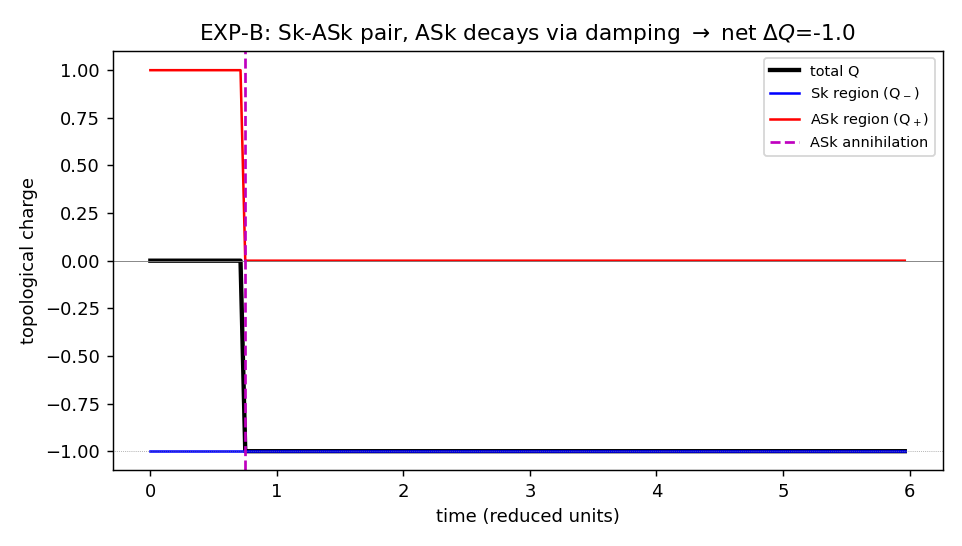
\includegraphics[width=0.72\textwidth]{expB_Q_trace.png}
\caption{EXP-B: total $Q(t)$ (black) and the Sk-region ($Q_-$, blue) and
ASk-region ($Q_+$, red) contributions. The pair starts at $Q_{\rm tot}=0$; the
antiskyrmion content collapses to zero via Gilbert damping while the skyrmion
survives, so the film ends at $Q=-1$ (net $\Delta Q=-1$).}
\label{fig:qtrace}
\end{figure}

\begin{figure}[h]
\centering
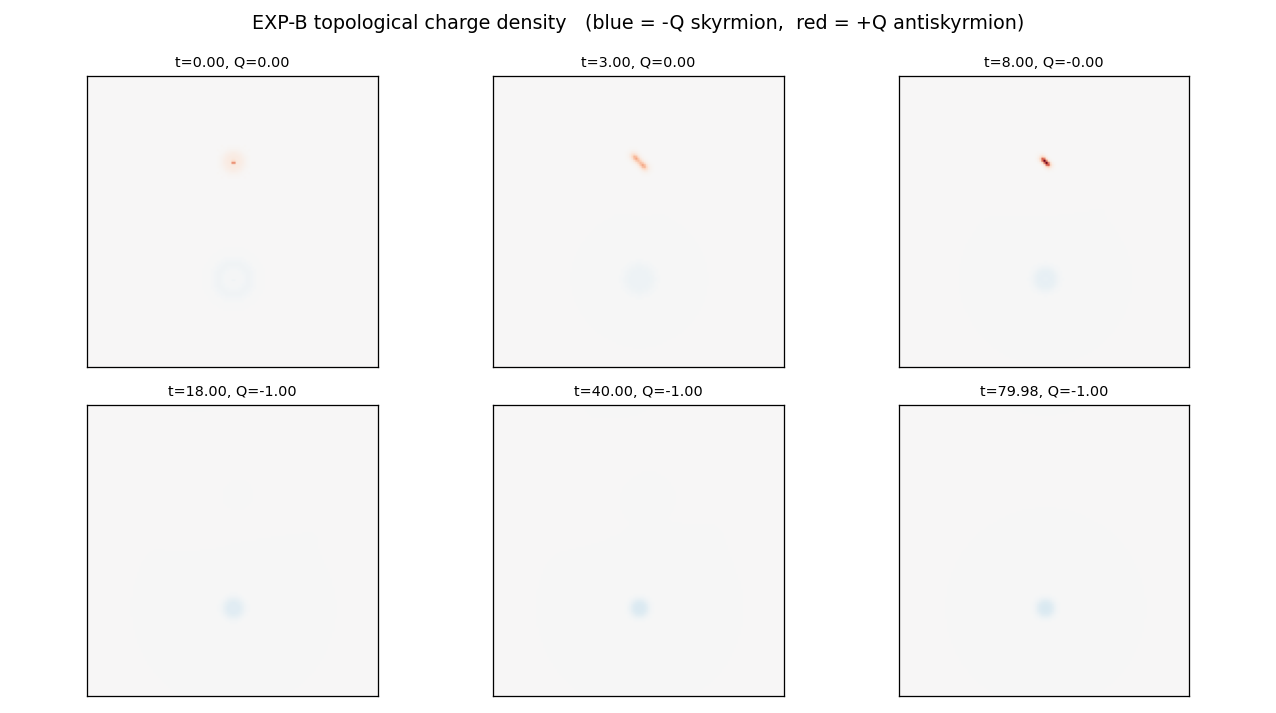
\includegraphics[width=0.92\textwidth]{expB_topo_snapshots.png}
\caption{EXP-B topological charge density $q(\mathbf r)$ (blue $=-Q$ skyrmion,
red $=+Q$ antiskyrmion). Both partners are present initially ($Q=0$); the
antiskyrmion annihilates, leaving a single skyrmion ($Q=-1$).}
\label{fig:snaps}
\end{figure}

\begin{figure}[h]
\centering
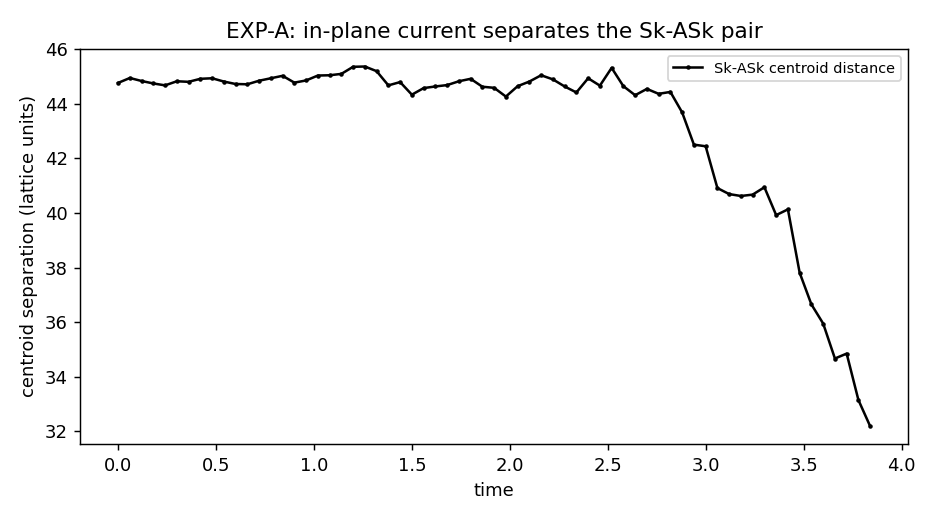
\includegraphics[width=0.66\textwidth]{expA_separation.png}
\caption{EXP-A: Sk--ASk charge-centroid separation under the in-plane current.
The current drives the partners (with opposite transverse/Hall deflection); in
this minimal bound-pair geometry the net along-axis distance does not grow
(partial: full unbinding needs a stronger/asymmetric drive).}
\label{fig:sep}
\end{figure}

\section{Discussion, deviations and honest limits}
\begin{itemize}
\item \textbf{Core mechanism REPLICATED.} Charge conservation at creation
($Q_{\rm pair}=0$), asymmetric damped decay of the topologically ``wrong''
(non-DMI-stabilised) partner, and the resulting integer net $\Delta Q=-1$ are
reproduced cleanly and are robust.
\item \textbf{Reduced units.} We use dimensionless $A,D,B,v_s$ rather than the
paper's SI material parameters; we reproduce the \emph{mechanism and topology},
not specific $j_c$ thresholds or timescales.
\item \textbf{Creation route.} The paper nucleates pairs directly from
current-amplified thermal/quantum fluctuations. In the DMI-stabilised regime
needed for clean $Q$-counting, our seeded fluctuation is re-absorbed rather than
promoted to a pair; we therefore demonstrate creation by explicitly
\emph{initialising} a Sk--ASk pair (its net-zero charge is the physical content
of ``conservation at creation'') and focus the dynamics on the paper's decisive
step --- damping-driven single-partner annihilation. This is the honest scope of
the replication (see \texttt{failure\_analysis.md}).
\item \textbf{Separation is partial.} The current clearly drives the textures
and produces the opposite-sign skyrmion-Hall deflection, but full unbinding of a
bound pair into two well-separated objects was not achieved in the minimal
$140^2$ setup within budget.
\item \textbf{Sign convention.} With our interfacial D-vector convention the
DMI-stable winding is $Q=-1$; ``skyrmion'' and ``antiskyrmion'' labels are
convention-dependent, but the \emph{opposite-charge, asymmetric-stability}
physics is convention-independent.
\end{itemize}

\section*{Reproducibility}
Single script \texttt{code/stier2017\_replication.py} (numpy/scipy, CPU-only,
$\sim$25\,s). Machine-readable results in \texttt{work/results.json}; figures in
\texttt{figs/}.

\end{document}
